\documentclass[11pt,a4paper]{article}
\usepackage{graphicx}
\graphicspath{ {images/} }
\usepackage{caption}
\usepackage{appendix}
\usepackage[top=1in, bottom=1in, left=1in, right=1in]{geometry}
\usepackage{multicol}
\setlength{\columnsep}{1cm}
\newenvironment{Figure}
  {\par\medskip\noindent\minipage{\linewidth}}
  {\endminipage\par\medskip}
\linespread{1.5}

\title{Investigation into Grading English Grammar}
\author{
        Martha Bellows 
\and
        Antoinette Bongiorno
\and 
	Brandon DiGiulio
}

\begin{document}
\maketitle

% --------------------------------------------------------------------
% --------------------------------------------------------------------
\section{Abstract}
% --------------------------------------------------------------------
% --------------------------------------------------------------------
Summary of paper. 

\pagebreak

\begin{multicols}{2}

% --------------------------------------------------------------------
% --------------------------------------------------------------------
\section{Introduction}
% --------------------------------------------------------------------
% --------------------------------------------------------------------
In the field of Automatic Text Summarization, there are two main categories of research: extractive and abstractive summarization. Extractive summarization describes the process of selecting contextually important sentences from the document and concatenating them to form a summary, while abstractive summarization aims to generate novel sentences that represent the main idea in a more concise manner. With advances in natural language processing and computer science, abstractive summarization and its newer counterpart, compressive summarization, have grown in popularity. Despite this growth in the field, it seems the methods used to evaluate progress have not scaled well, causing the community to continue to rely on human subjectivity as a metric in grading grammaticality and linguistics. In this paper we propose a model for evaluating grammaticality in a more objective and replicable way.


% --------------------------------------------------------------------
\subsection{Motivation}
% --------------------------------------------------------------------
In recent years, there has been research into using Integer Linear Programming for compressive summarization. In a paper by Li, Liu, Liu, Zhao, and Weng, we see the author's claim to make significant improvements in the linguistic quality of generated sentences using ILP and constituent parse trees. \cite{li2014} Curious to realize just how significant the improvements were, we looked into their method of measurement. In the paper, Li et al. cites that they ``invited [three] native English speakers to do the evaluation" \cite{li2014}. Taking note of the lack of replicability of this method, we recognized that there is a need for a more objective way to score the grammaticality and linguistic quality of sentences in order to further research in the growing field of Automatic Text Summarization. A more consistent method of grammaticality evaluation will help researchers measure the effectiveness of their systems, ranking them against competing research.

% --------------------------------------------------------------------
\subsection{NLP Community}
% --------------------------------------------------------------------
As research began with extractive summarization, it seems that the focus of Automatic Text Summarization is still on content and salience. In extractive summarization, the sentences that comprise the summary have not been altered in a way that could change their grammar, and assuming that the source document has correct grammar, there is not a need to score grammaticality. Due to this, the community standard for grading automatic summarization is the ROUGE metric \cite{yao2017}. This metric uses a comparison of n-grams between the summary to be evaluated and one or several human-written reference summaries, essentially scoring the content of the summary. Yao, Wan, and Xiao write that aside from content, evaluation on other aspects of summaries relies heavily on human judgement. At the Document Understanding Conference (DUC) which later became known as the Text Analysis Conference (TAC), the main conferences in the field, human judges are asked to rate different aspects of the summaries. This manual evaluation, on grammaticality, non-redundancy, clarity, and coherence, is said to be indispensable as there is no better solution at this time \cite{yao2017}.

This method of evaluation is used across the community. We see Li et al. asking a small sample of English native speakers to give a rating, on a scale from 1, bad, to 5, good, for both grammar and coherence \cite{li2014}. Woodsend and Lapata conduct their human judgement evaluations over the internet using Mechanical Turk, using a larger sample, of 54 volunteers. These self-reported native English speakers grade each summary for grammaticality and informativeness, on a scale of 1 to 5, after successful completion of comprehension questions \cite{woodsend2012}. In our research, we are curious as to why a better, more replicable and less subjective solution has not been developed, or been applied, before. At this time, there are commercial solutions that grade grammar, but none have been applied to this community that we saw in our research. In the model presented in this paper, we attempt to find a way to bridge this gap, so that automatic summarization research does not have to rely on the subjectivity of human judgement.


% --------------------------------------------------------------------
\subsection{Grammar}
% --------------------------------------------------------------------
In order to grade a summary on grammaticality, a definition for grammar needs to be established. Grammar is, simply put, a system of rules and syntax that defines how things should be written and spoken. Grammar gives communication an understood, defined meaning between two or more parties. These rules can be further defined using words' parts of speech and their relation to each other. ``We say a sentence is grammatically well formed when the adjacent words are in agreement with each other. That is, the parts-of-speech (POS) tags of adjacent words are mutually compatible, where the level of compatibility accounts to the degree of acceptance" \cite{Vadlapudi2010}. Using this, we can determine the importance of compatible combinations of POS tags in grading overall grammar.


% --------------------------------------------------------------------
% --------------------------------------------------------------------
\section{Parts of Speech Tagging}
% --------------------------------------------------------------------
% --------------------------------------------------------------------
Our idea is to develop a way to score the grammatical correctness of an input sentence based on the comparison of that sentence's POS tag sequence to a generated grammar rule set. This ruleset can be produced by processing a large number of grammatically correct sentences and analyzing these correct combinations of respective POS tags. By similarly processing automated text summaries into series of POS tags, we have the foundation for comparing a known set of correct sequences to these new, grammatically ungraded sentences. This grammaticality scoring method could someday replace human judgement in Automatic Text Summarization evaluation which will make this grading process more objective, reliable, and repeatable.


% --------------------------------------------------------------------
\subsection{Natural Language Toolkit}
% --------------------------------------------------------------------

In order to do the work of tagging sentences with parts of speech (POS) tags, we utilized the Natural Language Toolkit (NLTK) \cite{nltk}. NLTK is written in python and has many functions for natural language processing. In particular, we used NLTK in order to tokenize and tag sentences to build a text file of POS tag sequences. The tags used by NLTK is the Penn Treebank Tagset (Figure 1).

Other systems were considered such as RASP and an NLP system created by Stanford. RASP (Robust Accurate Statistical Parsing) is a system designed for syntactic annotation of free text \cite{briscoe}. It is implemented using C and Common Lisp and uses POS tags derived from the CLAWS tagset. The CLAWS tagset is comprised of over 130 tags, depending on the version, so it is much more extensive than the Penn Treebank Tagset. For example, the CLAWS tagset goes into finer detail with verbs specifying individual tags for the verbs to be, to do, and to have. It even goes so far as to break out each of these verbs to have a tag per verb tense. Because RASP uses a larger tagset, we deemed it would be beneficial to start with the simplest tagset available.

\begin{Figure}  
   \centering
   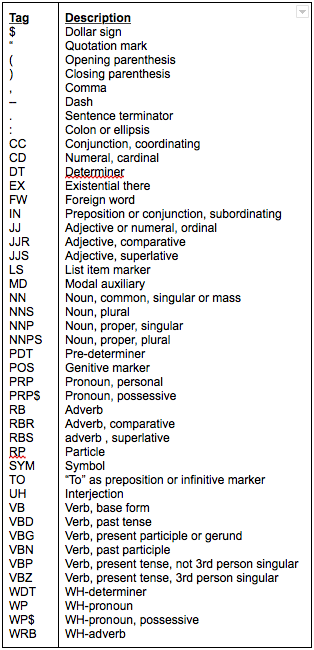
\includegraphics[width=\linewidth]{POStags}
   \captionof{figure}{Penn Treebank Tagset}
\end{Figure}   

The other system we considered is the NLP software available from The Stanford NLP group. Like NLTK, it uses the Penn Treebank tagset but instead of being implemented in python, they use Java. Ultimately, we decided to use python for our initial investigation because it is a good starting point. In addition, the documentation available from NLTK is extensive and easy to read.

% --------------------------------------------------------------------
\subsection{NLTK - Tagging Sentences}
% -------------------------------------------------------------------- 
In using NLTK, we are able to transform regular sentences into POS tags. There are four stages in this process from getting it from the initial sentence to a sentence with POS tags. Starting with initial sentences (1), it is necessary to convert it so each sentence is broken down into its individual sentences (2). This process is known as tokenizing sentences. The next step is to break each sentence into its individual words and punctuation which is called word tokenization (3). The final step is to tag each word in the sentence (4).

\begin{enumerate}
   \item Initial Sentence: `I went on a walk. It was nice outside.'
   \item Tokenize Sentence: [`I went on a walk.', `It was nice outside.']
   \item Tokenize Words: [[`I', `went', `on', `a', `walk', `.'], [`It', `was', `nice', `outside', `.']]
   \item Tag Words in Sentence: [(`I', `PRP'), (`went', `VBD'), (`on', `IN'), (`a', `DT'), (`walk', `NN'), (`.', `.')]
\end{enumerate}

These steps and the overall algorithm are further defined in Section 4.

% --------------------------------------------------------------------
\subsection{Project Gutenberg}
% --------------------------------------------------------------------
In order to build the rule set of correct tag sequences, literature from Project Gutenberg \cite{gutenberg} was used in addition to personally bought electronic literature. Project Gutenberg has a collection of free electronic books totaling more than 53,000. The majority of them are free because the books are considered public domain. A list of books used to create our file of tag sequences can be found in Appendix A. 

To use the books in our script for creating tag sequences, we had to use the .txt version in Project Gutenberg and convert our personal books from .mobi to .txt. The conversion of .mobi to .txt was done using the program Calibre. All files were then manually preprocessed and stripped of any text preceding or coming after the main text of the book. This includes title page information, letters by the author, acknowledgments, glossaries, etc.

Initially, we started only using four pieces of literature [Appendix A: 1, 4, 5, 9]. They were picked based on their popularity and their availability at Project Gutenberg. Because of their world-wide renown, proper grammar is assumed. Eventually we had to expand our data set so we added ten more books from Project Gutenberg [Appendix A: 2, 3, 6, 7, 8, 10, 11, 12, 13, 14]. This was still not sufficient to what we were trying to accomplish and reasoned that we should start including more recent pieces of literature. So far, the most recent publication we had was from 1911 [Appendix A: 11]. Since recent literature is not available on Project Gutenberg, we started using personally purchased literature [Appendix A: 15 - ].


% --------------------------------------------------------------------
% --------------------------------------------------------------------
\section{Algorithm}
% --------------------------------------------------------------------
% --------------------------------------------------------------------


% --------------------------------------------------------------------
\subsection{Generating Rule Set}
% --------------------------------------------------------------------

In this section, we go over how our algorithm generates its underlying rule set. Based on existing, assumed grammatically correct, pieces of work \cite{gutenberg}, we build a pseudo-database of correctly formed grammar combinations. Books are first read into memory by the application, one at a time. Using the Python NLTK library, each book is tokenized into separate sentences and then further tokenized into individual words per sentence. Each sentence is then treated separately, as each word contained within is tagged with the appropriate Part of Speech (POS) tag generated by the NLTK library. The result is a list of tuples each containing a word of the sentence and the POS tag. Since our algorithm will only care about the POS tags to check grammar, the original word is removed and all that remains is the sequence of POS tags for each sentence. 

Next the algorithm compares these new sequences with the current database to check for any existing matches. A binary search is done (the database is kept sorted) and if a match occurs, it will not be inserted so we avoid duplicated sequences. If there are no matches found at the end of the binary search, the sequence is added and the list sorted. Through this part of the overall algorithm, a ruleset to compare summaries and other sentences has been created.

\begin{Figure}  
   \centering
   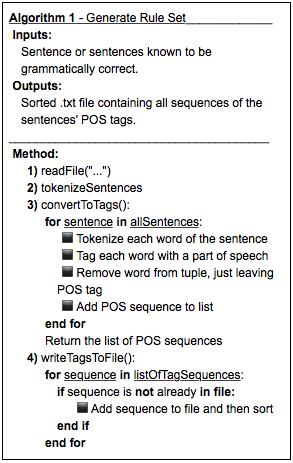
\includegraphics[width=\linewidth]{GenerateAlgorithm}
   \captionof{figure}{Algorithm 1 - Generating Rule Set}
\end{Figure}   

% --------------------------------------------------------------------
\subsection{Grading Against Rule Set}
% --------------------------------------------------------------------
In order to grade now against the aforementioned ruleset, we must now compare the grammar sequences of sentences to be graded with the ones that we already know to be correct. The new sentences must first be handled as the ones were in Section 4.1. They are first read and then processed using the NLTK library. Again, this tokenizes them into individual sentences, then words, and finally broken into sequences of POS tags.

It will next loop through each sequence generated from the summary or set of sentences and search for a matching sequence in the established ruleset. A binary search is performed on the ruleset and if a match is found, the sentence will receive a score of `1'. If a sentence does not find a matching sequence, it is assumed grammatically incorrect and thus will receive a score of `0.' Summing up all the scores across the input sentences, it is then divided by the total number of sentences to get an average score. This final score is the given grade for the summary's grammatical correctness.

\begin{Figure}  
   \centering
   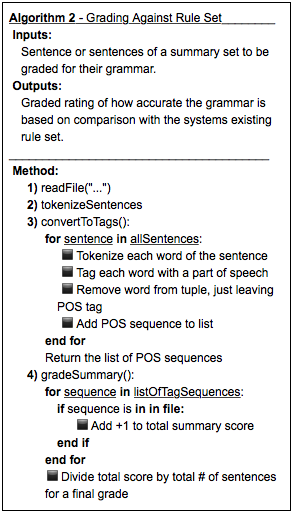
\includegraphics[width=\linewidth]{GradeAlgorithm}
   \captionof{figure}{Algorithm 2 - Grading Against Rule Set}
\end{Figure}   

% --------------------------------------------------------------------
% --------------------------------------------------------------------
\section{Results}
% --------------------------------------------------------------------
% --------------------------------------------------------------------
We expect that through grading summaries, grammatically correct sentences will have resulted with a score of `1' and grammatically incorrect sentences scored with a `0'. As the ruleset grows with the addition of more books, we also expect to see less false-negatives. 

The ruleset was initially established with the input of ten classical books from Project Gutenberg resulting in 56,025 unique POS tag sequences to be used for grammatical comparison and grading. Preliminary results showed that it would find and score correctly sentence structures that were known to be within the ruleset. However, the ruleset was not robust enough to cover everything and thus there were some known grammatically correct sentences that were still being given a score of `0.'

The ruleset was then built upon dramatically resulting in 414,461 unique POS tag sequences.

The algorithm was fed a control of one grammatically correct paragraph from one of the books included in our ruleset, one grammatically correct paragraph from an auto-summarizer, and one modified paragraph that was known to have a few grammatical mistakes.


% --------------------------------------------------------------------
% --------------------------------------------------------------------
\section{Limitations}
% --------------------------------------------------------------------
% --------------------------------------------------------------------
When creating the text file of correct POS tag sequences, it became apparent that it would continue to grow significantly no matter how many sentences were already included in the file. When added the ten books to it, it was apparent that there is not much overlap in sentence structure between each book. For example, the total number of sentences in all ten books is 58,895 while the tag sequences file has 56,025 sentences. This is a difference of only 2,870 meaning that between ten novels, there is only an overlap of about 5\%. This result is a clear example of the infiniteness of language. When discussing sentence construction in the NLTK documentation \cite{nltk}, they comment on how easy it is to ``extend sentences indefinitely." They go on to say ``it's not hard to concoct an entirely novel sentence, one that has probably never been used before in the history of the language." Because of the infiniteness of language, grammatically correct sentences that are not in the list of grammatically correct sequences is entirely possible.

Another limitation that will start happening with this method as more sentences are added is the text file will continue to grow. As mentioned, the number of tag sequences currently in the file is about 415,000 and that is only after utilizing about 55 books. As new works are added and the file grows, there will be an increasing need to optimize the algorithms for better storage and more efficient searching and sorting.

Limitations on books used\\

% --------------------------------------------------------------------
% --------------------------------------------------------------------
\section{Conclusion}
% --------------------------------------------------------------------
% --------------------------------------------------------------------
Conclusion

% --------------------------------------------------------------------
% --------------------------------------------------------------------
\section{Future Work}
% --------------------------------------------------------------------
% --------------------------------------------------------------------
In the future, we hope to further decrease the false negative rate by implementing a system to weigh grammaticality on a scale, versus scoring it completely correct or incorrect. We think that grading on a scale, meaning a sentence can be partially correct, would decrease the average number of false negatives. In addition, we think it will be important to experiment with additional tagging systems, mentioned in Section 3.1. Currently, we are using a very simple tagset. Our hypothesis was that the more simple the tag set, the more general sequences we would get, meaning more overlap in rule sequences. After reporting only about a 5\% overlap, we think that experimenting with more robust tagsets could have an significant impact on our results.

\newpage

\bibliography{references}
\bibliographystyle{ieeetr}

\end{multicols}

\pagebreak

\appendix
\appendixpage

% --------------------------------------------------------------------
% --------------------------------------------------------------------
\section{Literature}
% --------------------------------------------------------------------
% --------------------------------------------------------------------
Listed are the pieces of literature used in the created of the tag sequences file. Literature denoted with a "G" was obtained from Project Gutenberg. Anything denoted with a "P" indicates a book from one of the author's personal collection. The literature is ordered in the way it was added to the tag sequences file.

\begin{enumerate}
   \item Carroll, Lewis. (2008). \textit{Alice in Wonderland}. Urbana, Illinois: Project Gutenberg. Retrieved April 1, 2017, from http://www.gutenberg.org/ebooks/11. G.
   \item Bronte, Charlotte. (1998). \textit{Jane Eyre}. Urbana, Illinois: Project Gutenberg. Retrieved April 26, 2017, from http://www.gutenberg.org/cache/epub/1260/pg1260.txt. G. 
   \item Twain, Mark. (2004). \textit{The Adventures of Tom Sawyer}. Urbana, Illinois: Project Gutenberg. Retrieved April 26, 2017, from http://www.gutenberg.org/files/74/74-0.txt. G.
   \item Melville, Herman. (2001). \textit{Moby Dick}. Urbana, Illinois: Project Gutenberg. Retrieved April 1, 2017, from http://www.gutenberg.org/files/2701/2701-0.txt. G.
   \item Wilde, Oscar. (1994). \textit{The Picture of Dorian Gray}. Urbana, Illinois: Project Gutenberg. Retrieved April 1, 2017, from http://www.gutenberg.org/cache/epub/174/pg174.txt. G.
   \item Dickens, Charles. (1994). \textit{A Tale of Two Cities}. Urbana, Illinois: Project Gutenberg. Retrieved April 26, 2017, from http://www.gutenberg.org/cache/epub/174/pg174.txt. G.
   \item Gilman, Charlotte Perkins. (1999). \textit{The Yellow Wallpaper}. Urbana, Illinois: Project Gutenberg. Retrieved April 26, 2017, from http://www.gutenberg.org/cache/epub/1952/pg1952.txt. G.
   \item Austen, Jane. (1994). \textit{Emma}. Urbana, Illinois: Project Gutenberg. Retrieved April 26, 2017, from http://www.gutenberg.org/files/158/158-0.txt. G. 
   \item Austen, Jane. (1998). \textit{Pride and Prejudice}. Urbana, Illinois: Project Gutenberg. Retrieved April 1, 2017, from http://www.gutenberg.org/files/1342/1342-0.txt. G.
   \item Austen, Jane. (1994). \textit{Sense and Sensibility}. Urbana, Illinois: Project Gutenberg. Retrieved April 26, 2017, from http://www.gutenberg.org/cache/epub/161/pg161.txt. G.
   \item Barrie, J. M. (2008). \textit{Peter Pan}. Urbana, Illinois: Project Gutenberg. Retrieved April 28, 2017, from http://www.gutenberg.org/files/16/16-0.txt. G.
   \item Wells, H. G. (2004). \textit{The Time Machine}. Urbana, Illinois: Project Gutenberg. Retrieved April 28, 2017, from http://www.gutenberg.org/cache/epub/35/pg35.txt. G.
   \item Stevenson, Robert Louis. (2006). \textit{Treasure Island}. Urbana, Illinois: Project Gutenberg. Retrieved April 28, 2017, from http://www.gutenberg.org/cache/epub/120/pg120.txt. G.
   \item James, Henry. (1995). \textit{The Turn of the Screw}. Urbana, Illinois: Project Gutenberg. Retrieved April 28, 2017, from http://www.gutenberg.org/files/209/209-0.txt. G.
   \item Rowling, J. K. (1997). \textit{Harry Potter and the Sorcerer's Stone}. New York, NY: Scholastic Press. P.
   \item Rowling, J. K. (1999). \textit{Harry Potter and the Chamber of Secrets}. New York, NY: Scholastic Press. P.
   \item Rowling, J. K. (1999). \textit{Harry Potter and the Prisoner of Azkaban}. New York, NY: Scholastic Press. P.
   \item Rowling, J. K. (2000). \textit{Harry Potter and the Goblet of Fire}. New York, NY: Scholastic Press. P.
   \item Rowling, J. K. (2003). \textit{Harry Potter and the Order of the Phoenix}. New York, NY: Scholastic Press. P.
   \item Rowling, J. K. (2005). \textit{Harry Potter and the Half-Blood Prince}. New York, NY: Scholastic Press. P.
   \item Rowling, J. K. (2007). \textit{Harry Potter and the Deathly Hallows}. New York, NY: Scholastic Press. P.
   \item Gaiman, Neil. (2010). \textit{Stardust}. New York, NY: HarperTeen. P
   \item Bradbury, Ray. (2008). \textit{Fahrenheit 451}. Moline, IL: Moline Public Library. P.
   \item Bradbury, Ray. (2014). \textit{Something Wicked This Way Comes}. New York, NY: Harper. P.
   \item Card, Orson Scott. (2003). \textit{Speaker for the Dead}. Princeton, NJ: Princeton. P.
   \item Collins, Suzanne. (2008). \textit{The Hunger Games}. New York, NY: Scholastic Press. P.
   \item Collins, Suzanne. (2009). \textit{Catching Fire}. New York, NY: Scholastic Press. P.
   \item Collins, Suzanne. (2010). \textit{Mockingjay}. New York, NY: Scholastic Press. P.
   \item Fitzgerald, F. Scott. (1995). \textit{The Great Gatsby}. Ware: Wordsworth. P.
   \item Gaimain, Neil. (2014). \textit{Neverwhere}. New York, NY: Harper. P.
   \item Card, Orson Scott. (2009). \textit{Ender's Game}. New York, NY: Marvel Publishers. P.
   \item Gaiman, Neil. (2003). \textit{American Gods}. New York, NY: Perennial. P.
   \item Card, Orson Scott. (2002). \textit{Ender's Shadow}. New York, NY: Starscape. P.
   \item Card, Orson Scott. (2002). \textit{Children of the Mind}. New York, NY: Starscape. P.
   \item Herbert, Frank. (2005). \textit{Dune}. New York, NY: Ace Books. P.
   \item Lowry, Lois. (1993). \textit{The Giver}. Boston, MA: Houghton Mifflin. P.
   \item McEwan, Ian. (2002). \textit{Atonement: A Novel}. New York, NY: Nan A. Talese/Doubleday. P.
   \item Larson, Erik. (2003). \textit{The Devil in the White City: Murder, Magic, and Madness at the Fair that Changed America}. Princeton, NJ: Princeton. P.
   \item King, Stephen. (1977). \textit{The Shining}. New York, NY: Anchor. P.
   \item King, Stephen. (2006). \textit{Cell}. London: Hodder \& Stoughton. P.
   \item King, Stephen. (2004). \textit{Carrie}. New York, NY: Doubleday. P.
   \item King, Stephen. (2001). \textit{Bag of Bones}. New York, NY: Scribner. P. 
   \item Hemingway, Ernest. (2003). \textit{The Sun Also Rises}. New York, NY: Scribner. P.
   \item Hemingway, Ernest. (1995). \textit{A Farewell to Arms}. New York, NY: Scribner. P.
   \item Huxley, Aldous. (2007). \textit{Brave New World}. London: Grafton Books. P.
   \item Irving, John. (2002). \textit{A Prayer for Owen Meany: A Novel}. New York, NY: Modern Library. P.
   \item Jordan, Robert. (2000). \textit{The Eye of the World}. New York, NY: Tor Books, LLC. P.
   \item Mitchell, Margaret. (2007). \textit{Gone with the Wind}. New York, NY: Scribner. P.
   \item Kingsolver, Barbara. (2007). \textit{The Poisonwood Bible: A Novel}. New York, NY: Harper Perennial. P.
   \item Palahniuk, Chuck. (2005). \textit{Choke}. New York, NY: Anchor Books. P.
   \item Verne, Jules. (2006). \textit{Twenty Thousand Leagues Under the Sea}. Mineola, NY: Dover Publications. P.
   \item Verne, Jules. (2008). \textit{Journey to the Center of the Earth}. Vancouver, BC: Engage Books. P.
   \item Toole, John Kennedy. (2007). \textit{A Confederacy of Dunces}. New York, NY: Grove Press. P.
   \item Sanderson, Brandon. (2010). \textit{Mistborn: The Final Empire}. New York, NY: Tor Books. P.
   \item Tolkien, J. R. R. (2003). \textit{The Lord of the Rings: The Fellowship of the Ring}. Boston, MA: Houghton Mifflin. P.
   \item Steinbeck, John. (2006). \textit{The Grapes of Wrath}. New York, NY: Penguin Group. P.
   \item Salinger, J. D. (2010). \textit{The Catcher in the Rye}. New York, NY: Back Bay Books. P.
   \item Sagan, Carl. (2016). \textit{Contact}. New York, NY: Simon \& Schuster. P
   \item Pullman, Philip. (2001). \textit{The Golden Compass: His Dark Materials}. New York, NY: Knopf Books for Young Readers. P. 
   \item Pullman, Philip. (2001). \textit{The Subtle Knife: His Dark Materials}. New York, NY: Knopf Books for Young Readers. P. 
   \item Pullman, Philip. (2001). \textit{The Amber Spyglass: His Dark Materials}. New York, NY: Knopf Books for Young Readers. P. 
   
   
\end{enumerate}


\end{document}
